\subsection{Determining $\robotvelocity$}
\label{sec:desired_direction}

% \begin{minipage}{0.5\textwidth}
\begin{figure}[t]
    \centering
    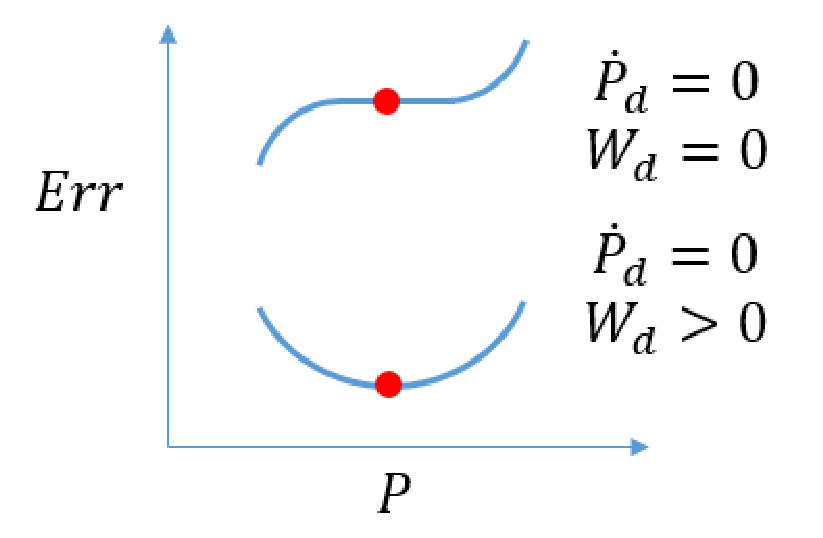
\includegraphics[width=1.8in]{error_graphs_modified}
    \caption{Top Line: moving the point does not change the error, thus the desired movement is zero, however, it is not important to achieve zero movement, thus $W_d = 0$.  Bottom Line: error is at a local minimum; thus moving the point increases error.}
    % \vspace{-0.2in}
    \label{fig:error_examples}
\end{figure}
% \end{minipage}
\begin{algorithm}[t]
    \caption{ErrorCorrection$(\deformconfig, \deformtarget)$}
    \begin{algorithmic}[1]
        \State $\deformvelocity_e \gets \boldsymbol 0_{\deformconfigspacesize \times 1}$, $\pseudoinverseweight_e \gets \boldsymbol 0_{\numdeformpoints \times 1}$
        \For{$i \in \{1,2,\dots,\numtargetpoints \}$}
            \State $k \gets \argmin_{j \in \{ 1,2,\dots,\numdeformpoints \}} \| \deformtarget_i - \deformconfig_j \|$
            \State $\deformvelocity_{e,k} \gets \deformvelocity_{e,k} + \deformtarget_i - \deformconfig_k$
            \State $\pseudoinverseweight_{e,k} \gets \max (\pseudoinverseweight_{e,k}, \| \deformtarget_i - \deformconfig_k \|)$
        \EndFor
        \State \Return $\{ \dot \deformconfig_e, \pseudoinverseweight_e \}$
    \end{algorithmic}
    \label{alg:error_correction}
\end{algorithm}
\begin{algorithm}[t]
    \caption{StretchingCorrection$(\relaxeddistancematrix, \lambda, \deformconfig)$}
    \begin{algorithmic}[1]
        \State $E \gets$ EuclidianDistanceMatrix$(\deformconfig)$
        \State $\deformvelocity_s \gets \boldsymbol 0_{3\numdeformpoints \times 1}$, $\pseudoinverseweight_s \gets \boldsymbol 0_{\numdeformpoints \times 1}$
        \State $\Delta \gets E - \relaxeddistancematrix$
        \For{$i \in \{1,2,\dots,\numdeformpoints \}$}
            \For{$j \in \{i+1,\dots,\numdeformpoints \}$}
                \If{$\Delta_{i,j} > \lambda$}
                    \State $v \gets \Delta_{i,j}(\deformconfig_j - \deformconfig_i)$
                    \State $\deformvelocity_{s,i} \gets \deformvelocity_{s,i} + \frac{1}{2}v$
                    \State $\deformvelocity_{s,j} \gets \deformvelocity_{s,j} - \frac{1}{2}v$
                    \State $\pseudoinverseweight_{s,i} \gets \max (\pseudoinverseweight_{s,i}, \Delta_{i,j})$
                    \State $\pseudoinverseweight_{s,j} \gets \max (\pseudoinverseweight_{s,j}, \Delta_{i,j})$
                \EndIf
            \EndFor
        \EndFor
        \State \Return $\{ \deformvelocity_s, \pseudoinverseweight_s \}$
    \end{algorithmic}
    \label{alg:stretching_correction}
\end{algorithm}
\begin{algorithm}[t]
    \caption{CombineTerms$(\deformvelocity_e, \pseudoinverseweight_e, \deformvelocity_s, \pseudoinverseweight_s)$}
    \begin{algorithmic}[1]
        \For{$i \in \{ 1,2,\dots,\numdeformpoints \}$}
            \State $\deformvelocity_{d,i} \gets \deformvelocity_{s,i} + \left( \deformvelocity_{e,i} - \proj_{\deformvelocity_{s,i}} \deformvelocity_{e,i} \right)$
            \State $\pseudoinverseweight_{d,i} \gets \pseudoinverseweight_{s,i} + \pseudoinverseweight_{e,i}$
        \EndFor
        \State \Return $\{ \deformvelocity_d, \pseudoinverseweight_d \}$
    \end{algorithmic}
    \label{alg:combine_terms}
\end{algorithm}
\begin{algorithm}[t]
    \caption{ObstacleRepulsion$(\obstacle, \beta)$}
    \begin{algorithmic}[1]
        \For{$\gripperindex \in \{1,2,\dots, \numgrippers\}$}
            \State $J_{p^g}, \dot x _{p^g}, d_g \gets$ Proximity$(\obstacle, \gripperindex)$
            \State $\gamma \gets e^{-\beta d_g}$
            \State $\robotvelocity_{c,g} \gets J_{p^g}^+ \dot x_{p^g}$
            \State $\robotvelocity_{c,g} \gets \frac{\maxgrippervelobstacle}{\| \robotvelocity_{c,g} \|} \robotvelocity_{c,g}$
            \State  $\robotvelocity_{\gripperindex} \gets \gamma \left( \robotvelocity_{c,g} + \left( \eye - J_{p^g}^+ J_{p^g} \right) \robotvelocity_\gripperindex \right) + (1-\gamma)\robotvelocity_\gripperindex$
        \EndFor        
        \State \Return $\robotvelocity$
    \end{algorithmic}
    \label{alg:obstaclerepulsion}
\end{algorithm}
\begin{algorithm}[t]
    \caption{Proximity$(\gripperindex, \obstacle)$ - reproduced from~\cite{Berenson2013}}
    \label{alg:proximity}
    \begin{algorithmic}[1]
        \State $d_\gripperindex \gets \infty$
        \For{$o \in \{1,2,\dots,|\obstacle|\}$}
            \State $p^\gripperindex, p^o \gets$ ClosestPoints$(\gripperindex, o)$
            \State $v \gets p^\gripperindex - p^o$
            \If{$\| v \| < d_\gripperindex$}
                \State $d_\gripperindex \gets \| v \|$
                \State $\dot x_{p^\gripperindex} \gets \frac{v}{\| v \|}$
                \State $J_{p^\gripperindex} \gets$ GripperPointJacobian$(\gripperindex, p^\gripperindex)$
            \EndIf
        \EndFor
        \State \Return $\{J_{p^\gripperindex}, x_{p^\gripperindex}, d_\gripperindex \}$
    \end{algorithmic}
\end{algorithm}

\subsubsection{Error Correction}

We build on previous work~\cite{Berenson2013}, splitting the desired deformable object movement into two parts: an error correction part and a stretching correction part. When defining the direction we want to move the deformable object to minimize error we calculate two values; which direction to move the deformable object points $\deformvelocity_e$ and the importance of moving each deformable object point $\pseudoinverseweight_e$. This is analogous to computing the gradient of error, as well as an ``importance factor'' for each part of the gradient. We need these weights to be able to differentiate between points of the object where the error function is a plateau versus points where the error function is at a local minimum~(Fig.~\ref{fig:error_examples}). Typically this is achieved using a Hessian, however our error function does not have a second derivative at many points. We use the \texttt{ErrorCorrection} (Alg.~\ref{alg:error_correction}) function to calculate these values. Each target point $\deformtarget_i \in \deformtarget$ defines a potential field, pulling the nearest point on the deformable object $\deformconfig_k$ towards $\deformtarget_i$. $\pseudoinverseweight_e$ is set to the maximum distance $\deformconfig_k$ is being pulled by any target point. This allows $\pseudoinverseweight_e$ to be insensitive to changes in discretization.

% \begin{wrapfigure}[21]{r}{0.5\textwidth}
% \begin{wrapfigure}[38]{r}{0.5\textwidth}
    % % \begin{minipage}{0.5\textwidth}
\begin{figure}[t]
    \centering
    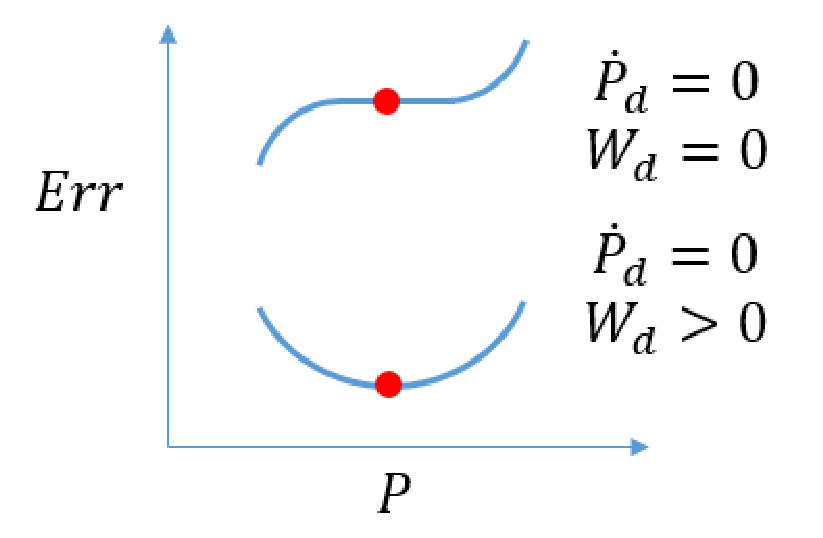
\includegraphics[width=1.8in]{error_graphs_modified}
    \caption{Top Line: moving the point does not change the error, thus the desired movement is zero, however, it is not important to achieve zero movement, thus $W_d = 0$.  Bottom Line: error is at a local minimum; thus moving the point increases error.}
    % \vspace{-0.2in}
    \label{fig:error_examples}
\end{figure}
% \end{minipage}
    % \vspace{-0.55in}
    % \begin{minipage}{0.5\textwidth}
        % \begin{algorithm}[t]
    \caption{ErrorCorrection$(\deformconfig, \deformtarget)$}
    \begin{algorithmic}[1]
        \State $\deformvelocity_e \gets \boldsymbol 0_{\deformconfigspacesize \times 1}$, $\pseudoinverseweight_e \gets \boldsymbol 0_{\numdeformpoints \times 1}$
        \For{$i \in \{1,2,\dots,\numtargetpoints \}$}
            \State $k \gets \argmin_{j \in \{ 1,2,\dots,\numdeformpoints \}} \| \deformtarget_i - \deformconfig_j \|$
            \State $\deformvelocity_{e,k} \gets \deformvelocity_{e,k} + \deformtarget_i - \deformconfig_k$
            \State $\pseudoinverseweight_{e,k} \gets \max (\pseudoinverseweight_{e,k}, \| \deformtarget_i - \deformconfig_k \|)$
        \EndFor
        \State \Return $\{ \dot \deformconfig_e, \pseudoinverseweight_e \}$
    \end{algorithmic}
    \label{alg:error_correction}
\end{algorithm}
        % \vspace{-0.57in}
        % \begin{algorithm}[t]
    \caption{StretchingCorrection$(\relaxeddistancematrix, \lambda, \deformconfig)$}
    \begin{algorithmic}[1]
        \State $E \gets$ EuclidianDistanceMatrix$(\deformconfig)$
        \State $\deformvelocity_s \gets \boldsymbol 0_{3\numdeformpoints \times 1}$, $\pseudoinverseweight_s \gets \boldsymbol 0_{\numdeformpoints \times 1}$
        \State $\Delta \gets E - \relaxeddistancematrix$
        \For{$i \in \{1,2,\dots,\numdeformpoints \}$}
            \For{$j \in \{i+1,\dots,\numdeformpoints \}$}
                \If{$\Delta_{i,j} > \lambda$}
                    \State $v \gets \Delta_{i,j}(\deformconfig_j - \deformconfig_i)$
                    \State $\deformvelocity_{s,i} \gets \deformvelocity_{s,i} + \frac{1}{2}v$
                    \State $\deformvelocity_{s,j} \gets \deformvelocity_{s,j} - \frac{1}{2}v$
                    \State $\pseudoinverseweight_{s,i} \gets \max (\pseudoinverseweight_{s,i}, \Delta_{i,j})$
                    \State $\pseudoinverseweight_{s,j} \gets \max (\pseudoinverseweight_{s,j}, \Delta_{i,j})$
                \EndIf
            \EndFor
        \EndFor
        \State \Return $\{ \deformvelocity_s, \pseudoinverseweight_s \}$
    \end{algorithmic}
    \label{alg:stretching_correction}
\end{algorithm}
    % \end{minipage}
    % \vspace{-0.62in}
% \end{wrapfigure}

\subsubsection{Stretching Correction}

Our algorithm for stretching correction is similar to that found in~\cite{Berenson2013}, with the addition of a weighting term $\pseudoinverseweight_s$, and a change in how we combine the two terms. We use the \texttt{StretchingCorrection} function (Alg.~\ref{alg:stretching_correction}) to compute $\deformvelocity_s$ and $\pseudoinverseweight_s$ based on a task-defined stretching threshold $\lambda \geq 0$. First we compute the distance between every two points on the object and store the result in $E$. We then compare $E$ to $D$ which contains the relaxed lengths between every pair of points. If any two points are stretched by more than $\lambda$, we attempt to move the points closer to each other. We use the same strategy for setting the importance of this stretching correction $\pseudoinverseweight_s$ as we use for error correction. When combining stretching correction and error correction terms (Alg.~\ref{alg:combine_terms}) we prioritize stretching correction, accepting only the portion of the error correction that is orthogonal to the stretching correction term for each point.

\subsubsection{Obstacle Avoidance}

% \begin{wrapfigure}{r}{0.5\textwidth}
    % \vspace{-0.55in}
    % \begin{minipage}{\columnwidth}
        % \vspace{-0.05in}
        % \begin{algorithm}[t]
    \caption{CombineTerms$(\deformvelocity_e, \pseudoinverseweight_e, \deformvelocity_s, \pseudoinverseweight_s)$}
    \begin{algorithmic}[1]
        \For{$i \in \{ 1,2,\dots,\numdeformpoints \}$}
            \State $\deformvelocity_{d,i} \gets \deformvelocity_{s,i} + \left( \deformvelocity_{e,i} - \proj_{\deformvelocity_{s,i}} \deformvelocity_{e,i} \right)$
            \State $\pseudoinverseweight_{d,i} \gets \pseudoinverseweight_{s,i} + \pseudoinverseweight_{e,i}$
        \EndFor
        \State \Return $\{ \deformvelocity_d, \pseudoinverseweight_d \}$
    \end{algorithmic}
    \label{alg:combine_terms}
\end{algorithm}
        % \vspace{-0.57in}
        % \begin{algorithm}[t]
    \caption{ObstacleRepulsion$(\obstacle, \beta)$}
    \begin{algorithmic}[1]
        \For{$\gripperindex \in \{1,2,\dots, \numgrippers\}$}
            \State $J_{p^g}, \dot x _{p^g}, d_g \gets$ Proximity$(\obstacle, \gripperindex)$
            \State $\gamma \gets e^{-\beta d_g}$
            \State $\robotvelocity_{c,g} \gets J_{p^g}^+ \dot x_{p^g}$
            \State $\robotvelocity_{c,g} \gets \frac{\maxgrippervelobstacle}{\| \robotvelocity_{c,g} \|} \robotvelocity_{c,g}$
            \State  $\robotvelocity_{\gripperindex} \gets \gamma \left( \robotvelocity_{c,g} + \left( \eye - J_{p^g}^+ J_{p^g} \right) \robotvelocity_\gripperindex \right) + (1-\gamma)\robotvelocity_\gripperindex$
        \EndFor        
        \State \Return $\robotvelocity$
    \end{algorithmic}
    \label{alg:obstaclerepulsion}
\end{algorithm}
        % \vspace{-0.57in}
        % \begin{algorithm}[t]
    \caption{Proximity$(\gripperindex, \obstacle)$ - reproduced from~\cite{Berenson2013}}
    \label{alg:proximity}
    \begin{algorithmic}[1]
        \State $d_\gripperindex \gets \infty$
        \For{$o \in \{1,2,\dots,|\obstacle|\}$}
            \State $p^\gripperindex, p^o \gets$ ClosestPoints$(\gripperindex, o)$
            \State $v \gets p^\gripperindex - p^o$
            \If{$\| v \| < d_\gripperindex$}
                \State $d_\gripperindex \gets \| v \|$
                \State $\dot x_{p^\gripperindex} \gets \frac{v}{\| v \|}$
                \State $J_{p^\gripperindex} \gets$ GripperPointJacobian$(\gripperindex, p^\gripperindex)$
            \EndIf
        \EndFor
        \State \Return $\{J_{p^\gripperindex}, x_{p^\gripperindex}, d_\gripperindex \}$
    \end{algorithmic}
\end{algorithm}
        % \vspace{-0.8in}
    % \end{minipage}
% \end{wrapfigure}
In order to guarantee that the grippers do not collide with any obstacles, we use the same strategy from~\cite{Berenson2013}, smoothly switching between collision avoidance and other objectives (see Alg.~\ref{alg:obstaclerepulsion}). For every gripper $\gripperindex$ and an obstacle set $\obstacle$ we find the distance $d_\gripperindex$ to the nearest obstacle, a unit vector $\dot x_{p_\gripperindex}$ pointing from the obstacle to the nearest point on the gripper, and a Jacobian $J_{p^\gripperindex}$ between the gripper's DOF and the point on the gripper as shown in Alg.~\ref{alg:proximity}. We then project the servoing motion from Eq.~\eqref{eqn:jacobianbackwardfunction} into the null space of the avoidance motion using the null space projector $\left(\eye - J_{p^g}^+ J_{p^g} \right)$. $\beta > 0$ sets the rate at which we change between servoing and collision avoidance objectives. $\maxgrippervelobstacle > 0$ is an internal parameter that sets how quickly we move the robot away from obstacles.

In principle the same null space avoidance can be used to prevent gripper-gripper collisions, but the tasks that we consider do not bring the the grippers close to each other in practice. Extensions to consider self collision and working with robot arms are discussed in Sec.~\ref{sec:real_robot}.